\section{Mathematical Methods}

A small number of mathematical methods which may not be familiar to the reader are used within this thesis. They are outlined below.

\subsection{K-means clustering}

\subsection{Principal Component Analysis}

\textit{A valuable primer on \gls{PCA} in relation to colour technology is available from \citet{tzeng_review_2005}.}

\glsreset{PCA}
\Gls{PCA} is a dimensionality reduction method, used to to reduce the number of variables within a dataset whilst retaining as much of the variance as possible, and often used to identify the correlated roots of variance.

Along with similar techniques, it is used extensively within the study of daylight \glspl{SPD}\citep{hernandez-andres_color_2001,ojeda_influence_2012,pant_estimating_2009,bui_group_2004,judd_spectral_1964,maloney_computational_1984,spitschan_variation_2016} and natural \glspl{SRF}\citep{maloney_computational_1984,dzmura_color_1992,maloney_evaluation_1986,maloney_color_1986,cohen_dependency_1964,ferrero_principal_2011,zhang_reconstructing_2008,kwon_surface_2007,agahian_reconstruction_2008,harifi_recovery_2008,parkkinen_characteristic_1989,vrhel_color_1992,fairman_principal_2004,ayala_use_2006,eem_reconstruction_1994-2,connah_multispectral_2006,shi_using_2002,morovic_metamer-set-based_2006}. 

In eras where the transmission of large datasets was troublesome, dimensionality reduction methods such as \gls{PCA} held value as a method to summarise a dataset, with the understanding that a reader could reconstruct a pseudo-dataset with minimal data-loss from the provided principal components. One such example is the work of \citet{judd_spectral_1964} where only the mean and first four 'characteristic vectors' are provided\footnote{This is not technically \gls{PCA} but the related technique of \citet{morris_objective_1954}.}. The data from \citet{judd_spectral_1964} is replotted in Figure \ref{fig:Judd} and it can be seen that for their dataset this description does seem to offer a sensible summary of the data: the shape of the mean can be seen, and it can be seen that the main variation further than 

\begin{figure}[htbp]
 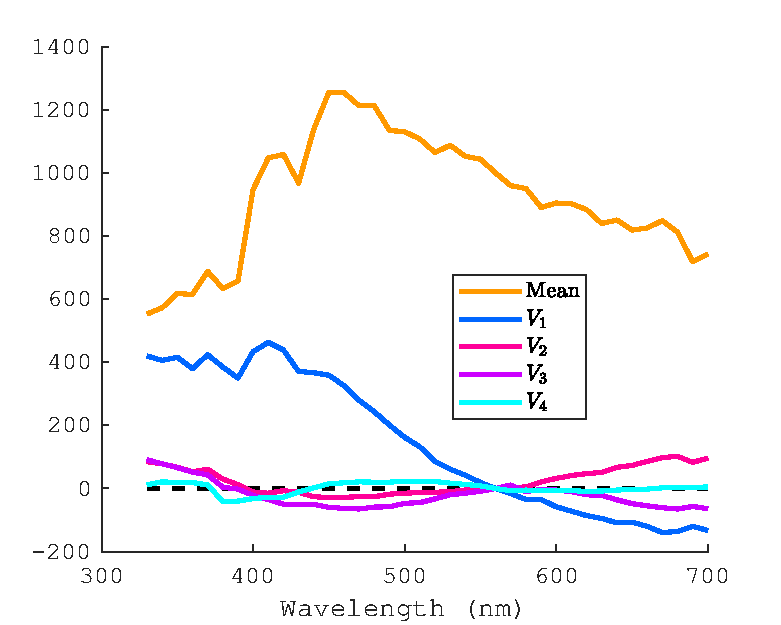
\includegraphics[max width=\textwidth]{figs/LitRev/Judd.pdf}
 \caption{The mean and first four characteristic vectors of \citet{judd_spectral_1964}.}
 \label{fig:Judd}
\end{figure} 